\section{Software Entwicklung}

\subsection{Allgemeine Begriffe}
\subsubsection{Schwierigkeiten}
	\begin{tabular}{ll}
	Essentielle Schwierigkeiten: & verursacht durch Komplexität des Problems \\
	Kontingente Schwierigkeiten: & selbst verursacht durch falsche Methoden, Mittel\\
	\end{tabular}
	
\subsubsection{Komplexität}
	\begin{itemize}
		\item Hauptproblem in der Softwareentwicklung
		\item \textbf{1. Gebot}: Halte die Komplexität im Griff.
	\end{itemize}
	
	\textbf{Bewältigung der Komplexität:}
		\begin{enumerate}
			\item Teile und herrsche \textit{"divide et impera"}
					\begin{itemize}
						\item Problem in Subprobleme aufteilen
						\item Unterteilung nach Problembereich (fachlich), Tätigkeiten und Zielen oder zeitlicher Abfolge
						\item Ansätze: möglichst eigenständige Teile (hohe Kohäsion) und möglichst geringe Abhängigkeiten (kleine Kopplung)
					\end{itemize}
			\item Abstraktion
					\begin{itemize}
						\item Definition: Weglassen von Aspekten und Details, die für den gegenwärtigen Zweck nicht wichtig sind.
					\end{itemize}
			\item Modelle
					\begin{itemize}
						\item Abstraktionen der realen Welt, z.B. Design-Modelle oder Domain-Modelle
					\end{itemize}
		\end{enumerate}
	
\subsubsection{Brook'sche Regel}
\textit{Adding manpower to a late project makes it later}  -  
Problem: Kommunikationsaufwand wird massiv erhöht.



\subsection{Vorgehensmodelle}

\subsubsection{Projektphasen}
	Alle Modelle basieren mehr oder weniger auf folgenden Projektphasen:
	\begin{itemize}
		\item Analyse
			\begin{itemize}
				\item Ziel: Man weiss mehr als vorher, Man weiss WAS entwickelt werden soll.
				\item Probleme, Ideen, Anforderungen aufnehmen
				\item Erstellen eines Pflichtenhefts
				\item \textit{doing the right things}
			\end{itemize}
		\item Design
			\begin{itemize}
				\item Ziel: Man weiss WIE das Produkt entwickelt werden soll
				\item Erstellen eines Grobentwurfs, Softwarekonzepts und von Detailentwürfen
				\item \textit{doing things right}
			\end{itemize}
		\item Implementierung
			\begin{itemize}
				\item Entwicklung des Sourcecodes anhand des Designs
			\end{itemize}
		\item Test
	\end{itemize}

\subsection{Wasserfall-Modell}
\begin{minipage}{11cm}
	\begin{itemize}
		\item linear (nicht iterativ)
		\item 1970 als fehlerhaftes, nicht funktionierendes System beschrieben
		\item Es gibt kein Zurück, alles muss beim ersten Mal richtig gemacht werden.
		\item Freigabe beim Abschluss jeder Phase
	\end{itemize}

	\subsubsection{Iterativer Wasserfall}
		\begin{itemize}
			\item = Kaskade
			\item Erweiterung des Wasserfalls um Korrekturschleifen
			\item In Realität durchführbar (nicht wie der reine Wasserfall)
			\item Man kann immer nur eine Phase zurück
		\end{itemize}
\end{minipage}
\begin{minipage}{8cm}
	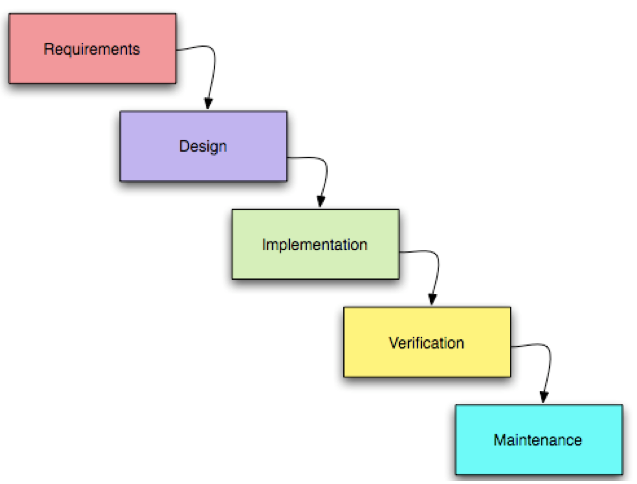
\includegraphics[width=8cm]{images/wasserfall_modell.png}
\end{minipage}

\subsection{V-Modell}
Grundidee: korrespondierende Tests \\
\begin{center}
	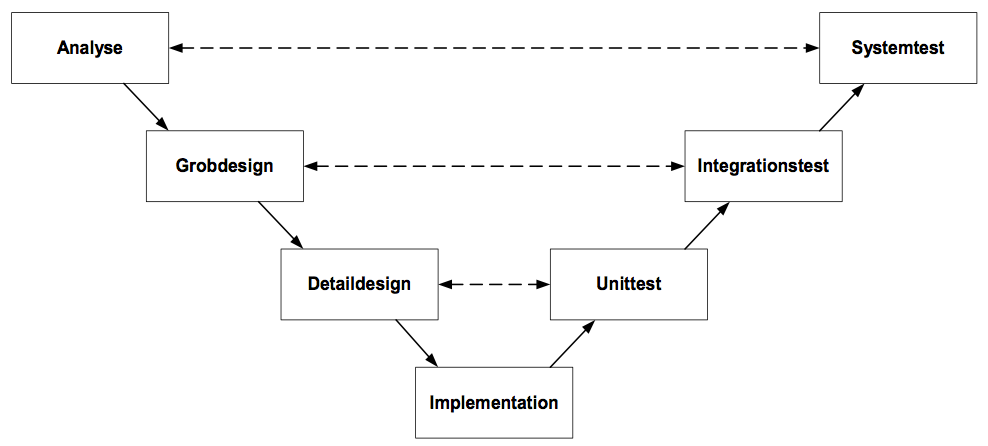
\includegraphics[width=12cm]{images/v_modell.png}
\end{center}

\subsection{Iterative / Inkrementelle Entwicklung}
\begin{minipage}{11cm}
	Grundidee: Software wird in einzelnen Schritten erstellt. \\
	
	\textbf{Inkrementell:}
		\begin{itemize}
			\item Resultat in Schritten entwickeln
			\item Jeder Schritt ist Teil des Endresultats
		\end{itemize}
	\textbf{Iterativ:}
		\begin{itemize}					
			\item Erste Version entwickeln
			\item In weiteren Schritten bessere Versionen erstellen
		\end{itemize}
\end{minipage}
\begin{minipage}{8cm}
	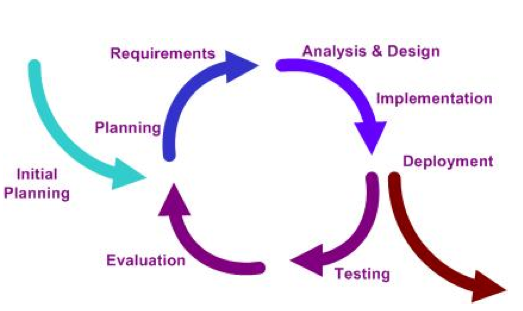
\includegraphics[width=8cm]{images/iterative_entwicklung.png}
\end{minipage}

\newpage %TODO: Newpage entfernen
\subsubsection{Spiralmodell}
Entwickelt von Barry Böhm, 1988
\begin{center}
	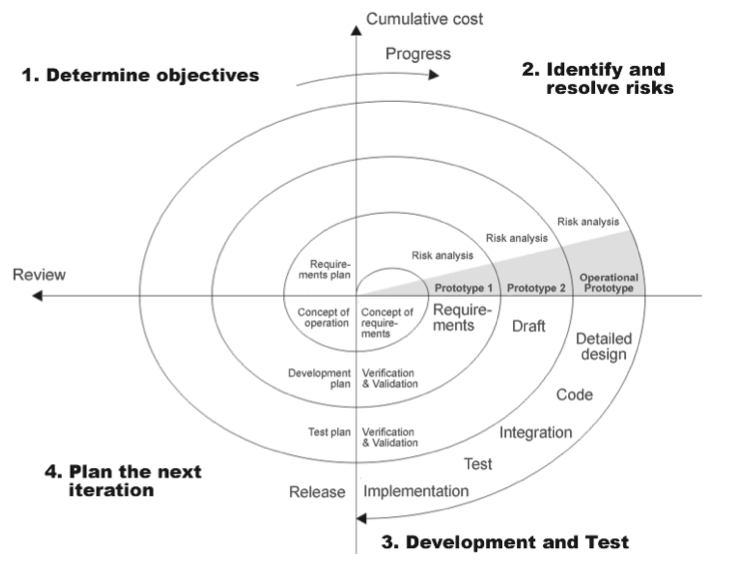
\includegraphics[width=12cm]{images/spiral_modell.png}
\end{center}

\subsection{Agile Softwareentwicklung}
\begin{itemize}
	\item Gegenbewegung zur herkömmlichen schwerfälligen, bürokratischen Softwareentwicklung
	\item agile = flink, beweglich
	\item Individuen und Interaktionen gelten mehr als Prozesse
	\item Grundlagen: Extreme Programming (Kent Beck, 1999); Agiles Mainfest (2001)
\end{itemize}

Agile Softwareentwicklung besteht aus:
\begin{enumerate}
	\item Agile \textit{Werte} bilden das Fundament.
	\item Agile \textit{Prinzipien} sind Handlungsgrundsätze, die auf agilen Werten basieren.
	\item Agile \textit{Methoden} sind konkrete Verfahren, die sich auf agile Werte und Prinzipien stützen.
	\item Agile \textit{Prozesse} sind die Zusammenfassung agiler Methoden. 
\end{enumerate}

\subsubsection{XP (Extreme Programming)}
\begin{minipage}{12cm}
	\begin{itemize}
		\item Bekanntester agiler Prozess
		\item Nach Buch ``Extreme Programming'' von Kent Beck (1999)
	\end{itemize}
\end{minipage}
\begin{minipage}{6cm}
	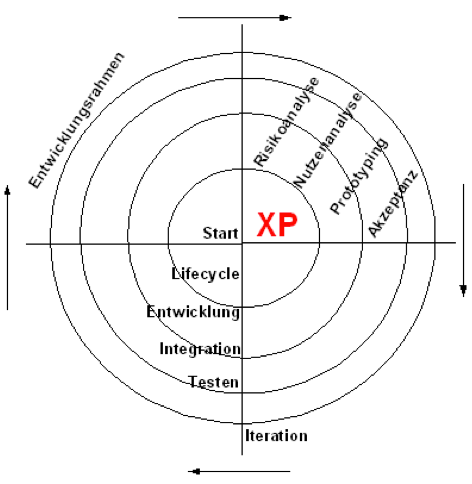
\includegraphics[width=6cm]{images/extreme_programming.png}
\end{minipage}

\subsubsection{Scrum}
\begin{minipage}{11cm}
	\begin{itemize}
		\item = ``Gedränge''
		\item Vorgestellt auf OOPSLA '95
		\item Basis: Sprints von 15-30 Tagen
	\end{itemize}
\end{minipage}
\begin{minipage}{8cm}
	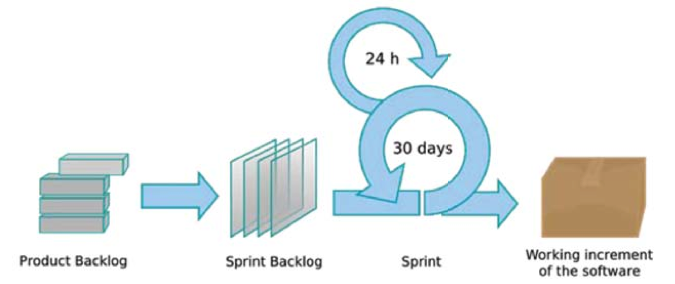
\includegraphics[width=8cm]{images/scrum.png}
\end{minipage}

\subsection{Objektorientierte Softwareentwicklung}
Grundidee: Modelle auf allen Stufen: OO-Analyse $\rightarrow$ OO-Design $\rightarrow$ OO-Implementation. Objekte entsprechen in der Regel realen Dingen; Änderungen werden daher weniger häufig und einfacher. \\

Kriterien für die Wahl des Modells:
\begin{itemize}
	\item Verfügbarkeit der Ressourcen
	\item Projektkomplexität
	\item Zeitpunkt von Änderungen (diskret, laufend)
	\item Qualität der Anforderungsdefinitionen
	\item Stabilität bzw. Volatilität der Anforderungen
\end{itemize}